\section{System Overview}
\label{sec-system-overview} 
We implemented a holistic system for shoulder surfing, with the neural network as core, on a smartphone to verify the efficiency of our model. It iterates through the following steps: 

\vspace{1mm}
\noindent
\textbf{Input:} Under guidance of the attacker, The smartphone will zoom in, take focus, and take 20 images with burst mode of the target screen. Note that zooming is only for easier interaction and focusing, and to utilize the telephoto lenses and optical zoom, if available, as digital zooming do not put in any extra data; On traditional phones with only digital zooming, the photo-taking will be with 1x zoom, and on phones with optical zooming, 5x to 10x zoom, depending on the optical zooming range. This way information on the images will be more compact and easier to comprehend by neural networks.

\vspace{1mm}
\noindent
\textbf{Alignment:} The images are then aligned to mitigate the shifts between frames caused by hand tremor or movements from the lenses, as cameras with optical lenses will occasionally shift slightly across time due to the movements of its inner mechanism. Luckily, in our scenario the target is a glowing screen whose edges are easily distinguishable in most cases, and we use them as reference to align our images. The images are also spun to make the text horizontal in the process. The screen is cropped out and the rest of the image abandoned.


\vspace{1mm}
\noindent
\textbf{Adjustment:} The lines of text(or stuff differing from the background color of the screen) will be carved out for processing, to reduce the workload of the network. The characters are normally around 10x10 pixels in the photos, and the carved segments will leave 2 pixels of padding on all sides to avoid mutilating the character; A certain amount of error is allowed, but if the size of the text is too small or too large, the neural network will not be able to extract features normally, so the images will be zoomed to the right size (and the zooming of the camera lens in the Input phase will be adjusted accordingly).


\vspace{1mm}
\noindent
\textbf{Processing:} As our network accepts only 9x9 patches, we will process all the 9x9 patches among the input photo with our multi-frame super resolution network to generate 36x36 images (4x upscaling). The input is RGB colored, while the output, as we are not interested in color, is black and white. In this way, we generate upscaled image segments of all the characters on the target screen. The three calculation processes (Alignment, Adjustment, Processing) runs parallel to the input process, so that once a batch of input images is available, they can be calculated and displayed on screen with a slight lag while the attacker can start to collect the next batch at the same time.
		
\vspace{1mm}
\noindent
\textbf{Output:} The outputs of our SR network, the 36x36 patches, are then merged into a whole. The overlapping pixels are thus processed: among all the outputs containing this pixel, we collect these values, remove outliers, and use their average as the result. As we only carve out the texts on the phone and process them, we will then insert these high-res texts back to their original locations on one of the input images, and display the patched image to the attacker (An illustration can be found in Fig.~\ref{illustration_of_system}).

These steps are repeatedly executed to enable the attacker to monitor the victim at an interval of a few seconds. At critical times requiring continuous monitoring so as not to miss transient display, e.g. password entering, the system can simply lengthen the input phase across that period and process the data afterwards. The workflow of our system is shown in Figure~\ref{fig-workflow}.
\begin{figure}
  \centering
     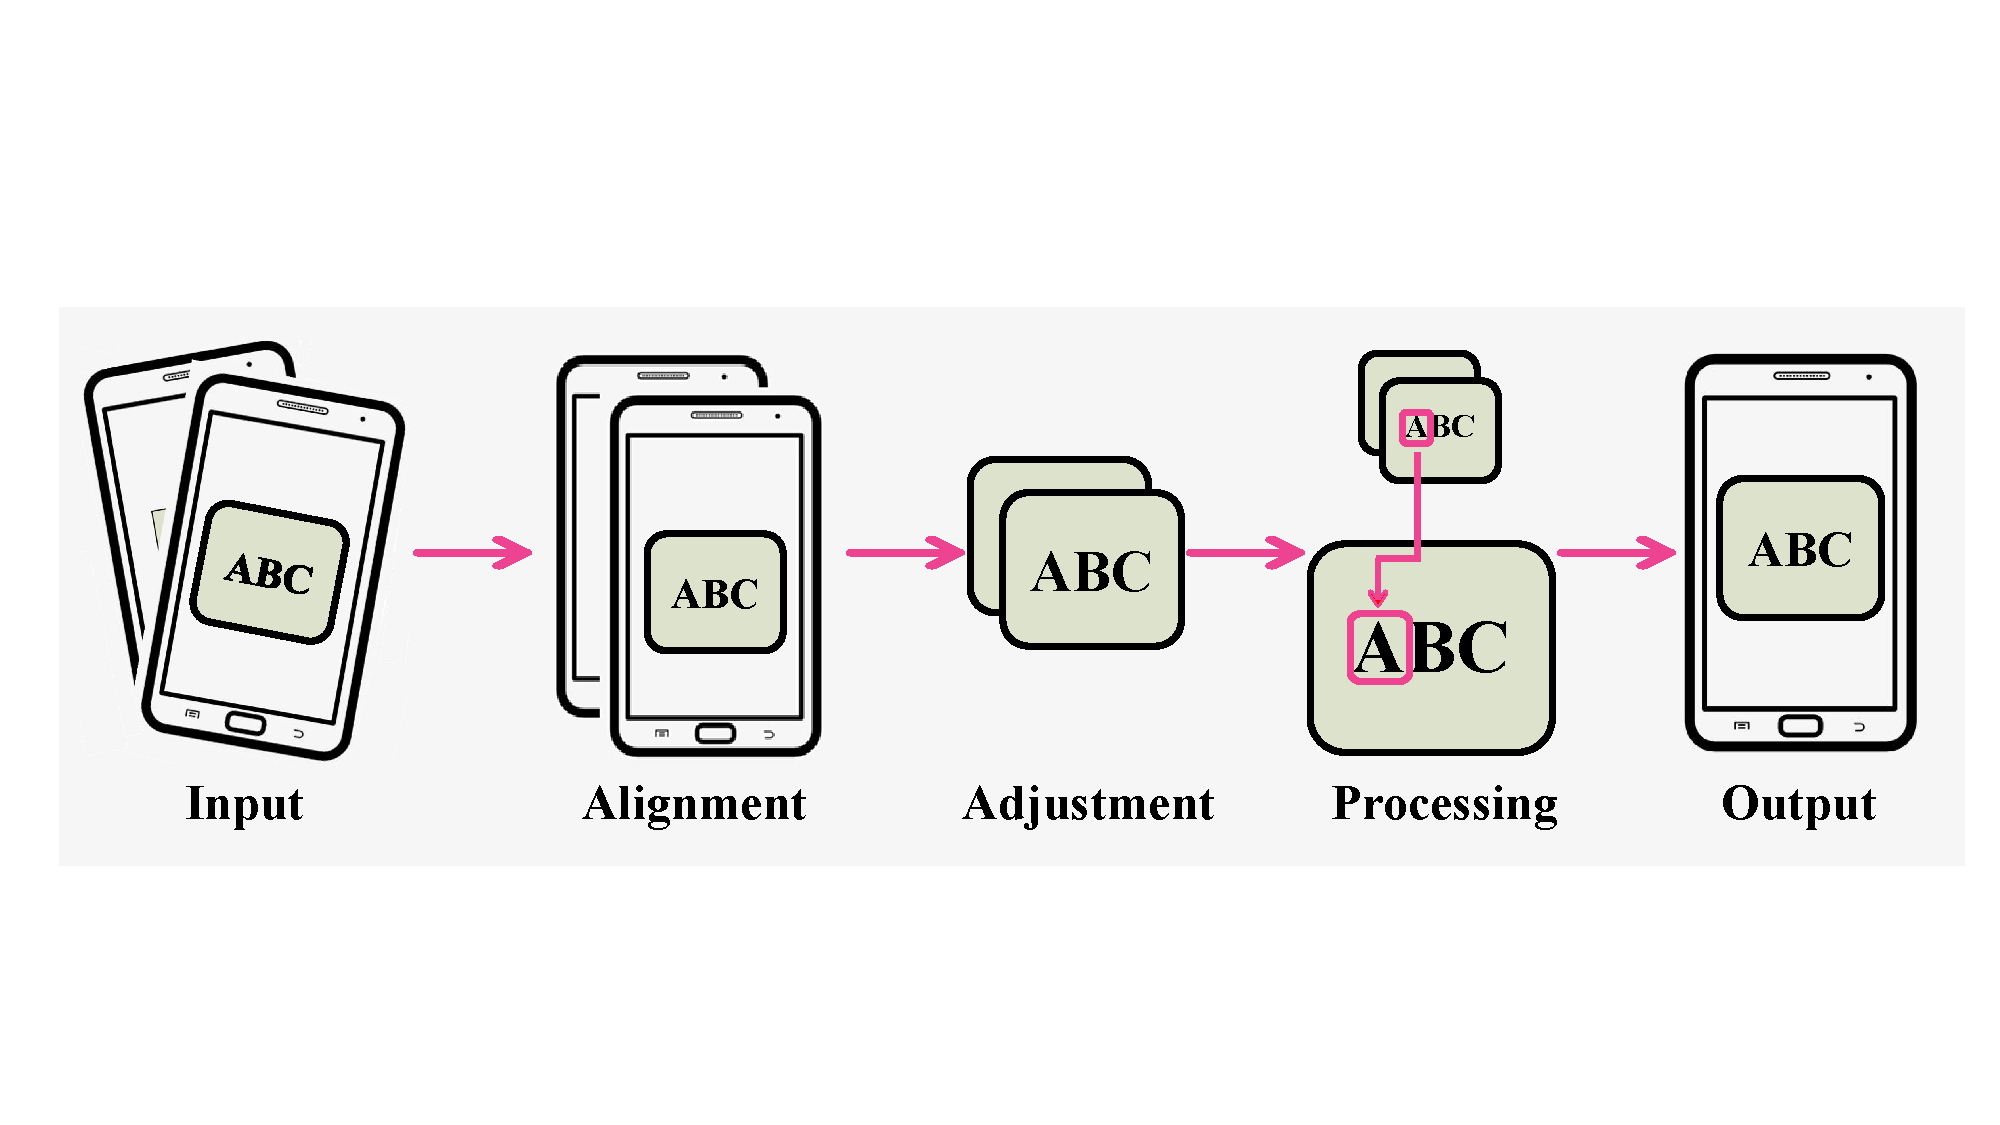
\includegraphics[width=0.48\textwidth]{./pic/workflow_cl.pdf}
     \caption{Illustration of the workflow of \textsf{SRPeek}.}
     \label{fig-workflow}
\end{figure}


